\documentclass[10pt]{beamer}

\usetheme{metropolis}
\usepackage{appendixnumberbeamer}

\usepackage{booktabs}
\usepackage{graphicx}
\usepackage{subcaption}
\usepackage[scale=2]{ccicons}
\usepackage{gensymb}

\usepackage{pgfplots}
\usepgfplotslibrary{dateplot}

\usepackage{xspace}
\newcommand{\themename}{\textbf{\textsc{metropolis}}\xspace}

\DeclareMathOperator*{\argmin}{arg\,min}
\DeclareMathOperator*{\argmax}{arg\,max}

\graphicspath{{./images/}}

\title{Machine Vision for Crack Detection}
\subtitle{Fault identification in solar panels and wind turbine blades}
\date{\today}
\author{Jerome Wynne}
\institute{University of Bristol, DNV-GL}

\begin{document}

\maketitle

\begin{frame}{Table of contents}
  \setbeamertemplate{section in toc}[sections numbered]
  \tableofcontents[hideallsubsections]
\end{frame}

%% >> Problem Description << %%
\section{Problem Description}
%% Problem Description: 1. Where are the images coming from?
\begin{frame}[fragile]{Problem Description}
	DNV have recently begun inspecting wind turbines using drones.
	
	 The footage captured is manually reviewed in search of damage.
	
	\textbf{Our work}
	
	We sought to develop a computational model capable of identifying damage automatically.

	\begin{figure}
		\includegraphics[width=0.5\textwidth]{stock_drone_inspector.jpg}
		\caption{Automated turbine inspection can alleviate the personal risk, tedium, and expense of manual turbine inspection.}
	\end{figure}
	
\end{frame}

%% Problem Description: 2. Data introduction
\begin{frame}[fragile]{Problem Description}
	The drones captured visible and thermal video, along with point cloud data using an on-board lidar scanner.
	
	\textbf{Defects of interest}
	\begin{itemize}
		\item[-] Cracks
		\item[-] Delaminated regions
	\end{itemize}
	
	\begin{figure}
		\begin{subfigure}[b]{0.35\textwidth}
			\includegraphics[width=\textwidth]{sample_blade.jpg}
			\caption{Image from the dataset.}
		\end{subfigure}
		\qquad
		\begin{subfigure}[b]{0.35\textwidth}
				\includegraphics[width=\textwidth]{sample_blade_zoomed.png}
			\caption{Crack on leading edge.}
		\end{subfigure}
	\end{figure}
	
\end{frame}

%% Problem Description: 3. Complicating factors
\begin{frame}[fragile]{Problem Description}
	\textbf{Complicating factors}
	\begin{itemize}
		\item[-] Redundant information ($1400 \times 1400$ images)
		\item[-] Dirt
		\item[-] Background
		\item[-] Lighting conditions
		\item[-] Dynamic pathfinding
		\item[-] Camera focus
		\item[-] Junk on lens (e.g. water droplets, debris)
	\end{itemize}
	
	Exploratory work was conducted on a toy problem that was thought more tractable.
\end{frame}


%% Problem Description: 4. Toy problem
\begin{frame}[fragile]{Problem Description}
	\textbf{Toy problem}
	
	 Detect cracks in images of solar panels.
	 
	\begin{figure}
		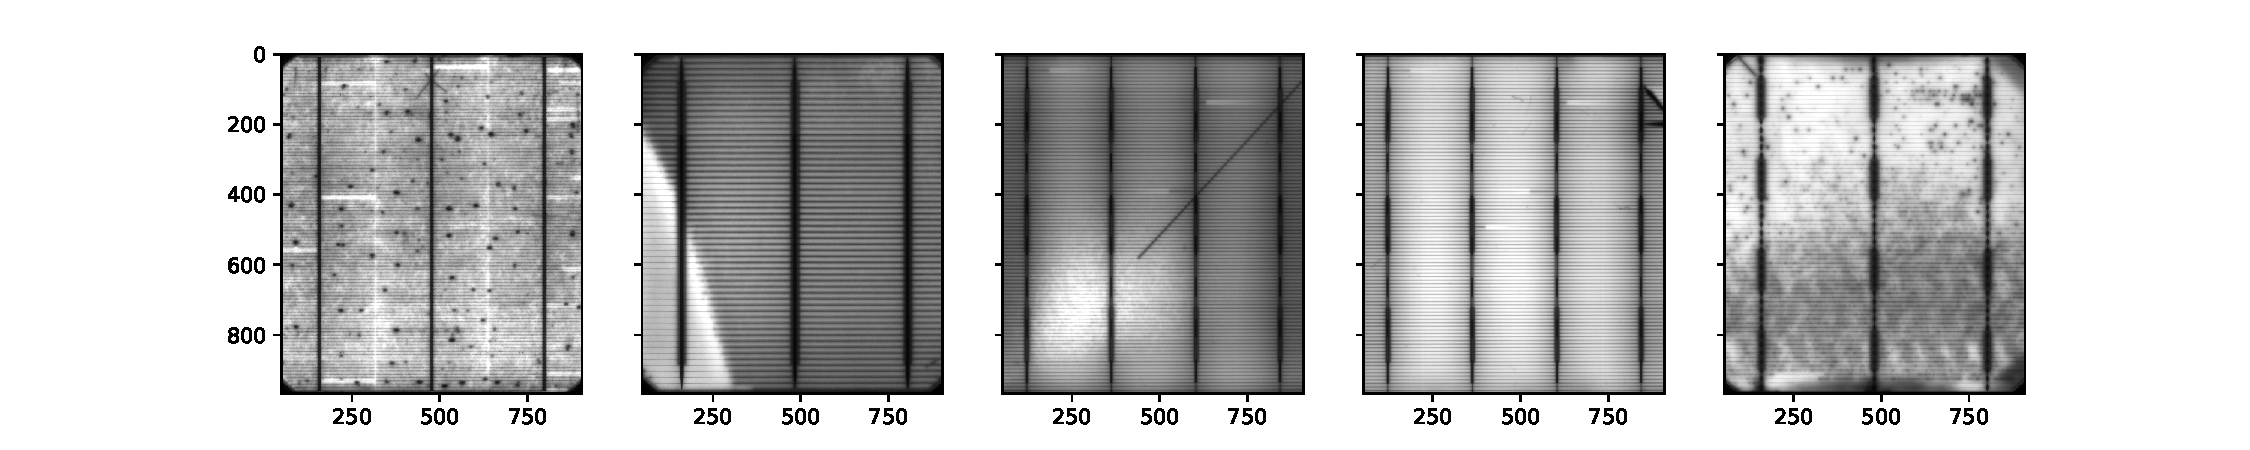
\includegraphics[width=0.7\textwidth]{sample_panels.png}
		\caption{A sample of scanned panels. Cracks are dark lines oriented at $\approx 45\degree$.}
	\end{figure}
\end{frame}

%% Problem Description: 5. Complicating factors of toy problem
\begin{frame}[fragile]{Problem Description}
	\textbf{Complicating factors}
	\begin{itemize}
		\item[-] Handling large-ish images ($\approx 965 \times 965$)
		\item[-] Low-frequency intensity variation due to delamination
		\item[-] High-frequency intensity variation due to cells
		\item[-] Other noise - hail damage, scratches, panel models, debris in scanner
		\item[-] Variation between panel models
		\item[-] Small dataset (52 images, not all of which were cracked)
	\end{itemize}
\end{frame}


%% >> Modeling Strategy << $$
\section{Modeling Strategy}

%% Modeling Strategy: 1. Approach
\begin{frame}[fragile]{Modeling Strategy}
	\textbf{Approach}
	\begin{itemize}
	\item[-]Supervised classification/regression problem.
	\item[-]Manual and learned representations of the images were developed.
	\item[-]A variety of discriminative and generative models considered.
	\end{itemize}
	\textbf{Desirable model attributes}
	\begin{itemize}
		\item[-] Accurate
		\item[-] Sensitive
		\item[-] Probabilistic
		\item[-] Localizes damage
	\end{itemize}
\end{frame}

%% Modeling strategy: 2. Labeling
\begin{frame}[fragile]{Modeling Strategy}
	\textbf{Labeling}
	
	 Binary masks were created indicating which pixels constituted a crack segment.
	
	\textbf{Ground truth subjectivity}
	
	 Cracks and scratches were difficult to distinguish: In general, the latter were fainter and had more curvature.
	\begin{figure}
		\includegraphics[width=0.6\textwidth]{sample_mask.pdf}
		\caption{A panel and its associated binary mask.}
	\end{figure}
\end{frame}

%% Modeling strategy: 3. Loss function
\begin{frame}[fragile]{Modeling Strategy}
	\textbf{Loss function}
	
	Empirical per-pixel classification error rate:
	\[
		J(\theta) = \mathbb{E}_{\mathbf{x}, y \sim p_{train}} |f(\mathbf{x};\theta) - y|
	\]
	Where $p_{train}$ is the sampling distribution described by the training data, and $f$ is our learned function mapping from a set of input features $\mathbf{x}$ to a class $y \in \{0, 1\}$, parameterized by the set $\theta$.
	
	\textbf{Surrogate Loss Function}
	
	To improve our classifier's ability to discriminate between classes, we adopted cross-entropy as a surrogate measure of loss:
	\[
		J^*(\theta) = \mathbb{E}_{\mathbf{x}, y \sim p_{train}} -\Big[(1-y)\log[1 - q(\mathbf{x}; \theta)] + y\log[ q(\mathbf{x}; \theta)]\Big]
	\]
	Where $q(\mathbf{x};\theta)$ denotes the probability our learned function assigns to $\mathbf{x}$ being a positive instance.
\end{frame}


%% >> Experimental Procedure << %%
\section{Experimental Procedure}
%% Ex procedure: 1. Preprocessing procedure + training protocol
\begin{frame}{Experimental Procedure}
\textbf{Vanilla preprocessing procedure}
  \begin{itemize}
  	\item[-] Resize the images ($965 \times 965 \rightarrow 200 \times 200$).
  	\item[-] Apply a global per-pixel mean subtraction and scaling by standard deviation (a.k.a. \emph{whitening})\footnote{whitening encourages numerical stability and suppresses common artifacts.}
\end{itemize}

\textbf{Training protocol}
\begin{itemize}
  	\item[-] Compute parameters with closed-form expressions over the entire training set.
  	\item[-] On-line minibatch training - gather a balanced minibatch across all pixels only as needed (1.5m+ negative examples, $<$ 10k positive examples).
  	\item[-] Apply basic patch augmentations (flipping, rotation, intensity shifts).
  \end{itemize}
\end{frame}

%% Exp procedure: 2. Implementation
\begin{frame}[fragile]{Experimental Procedure}
\textbf{Implementation}

TensorFlow was chosen as a development platform. Very good reasons for this\footnote{at a cost of greater verbosity + cryptic error messages}:
\begin{itemize}
	\item Flexible modeling environment
	\item Excellent diagnostic and logging tools
	\item GPU support
\end{itemize}
\end{frame}


%% >> Models & Representations << %%
\section{Models \& Representations}

%%  Models: 1. Problem attributes
\begin{frame}{Models \& Representations}
	\textbf{Crack attributes}
	\begin{itemize}
		\item Continuous
		\item Small aspect ratio
		\item Dark (constant intensity)
		\item Generally propagates diagonally
		\item Near borders
		\item ...
	\end{itemize}
	
	\textbf{Non-crack attributes}
	\begin{itemize}
		\item Horizontal/vertical gradients, or a mush of gradients (in the case of circular elements)
		\item Higher intensity values than crack
		\item Patterned
		\item Variable intensity
		\item ...
	\end{itemize}
\end{frame}

%%  Models: 2. Models
\begin{frame}{Models \& Representations}
	\textbf{Models implemented}
	\begin{itemize}
		\item Gaussian discriminant analyzers.
		\item Convolutional neural networks.
			\begin{itemize}
				\item Batch normalization units
				\item Spatial transformer subnetworks
				\item Expanded input feature spaces
			\end{itemize}
		\item Canned \texttt{sklearn} classifiers.
	\end{itemize}
	
	\textbf{Models explored}
	\begin{itemize}
		\item Relaxation labelers
		\item Hidden Markov models
		\item Markov random fields
	\end{itemize}
\end{frame}



%% >> Results << %%
\section{Experimental Results}

\begin{frame}{Experimental Results}
	\textbf{Gaussian discriminant analyzer}
	
	As a point of reference, we attempted to model class-conditional pixel intensity variation using a multivariate normal distribution over a patch of pixels:
	\[
		\text{Pr}(\mathbf{x}|y = k, \boldsymbol{\mu}_k, \mathbf{\Sigma}_k) = \text{Norm}_{\mathbf{x}}[\mathbf{x}, \boldsymbol{\mu}, \mathbf{\Sigma}]
	\]
	Where $\boldsymbol{\mu}_k, \mathbf{\Sigma}_k$ are the class mean and covariance respectively. A Bernoulli prior was used, parameterized by the base rate $\lambda$. The maximum likelihood estimate of these parameters was taken.
	
	 For inference, the maximum \emph{a posteriori} class was taken:
	\[
		\hat{y} = \argmax_k \Big[\text{Pr}(\mathbf{x}|y = k, \boldsymbol{\mu}_k, \mathbf{\Sigma}_k) \cdot \text{Pr}(y = k, \lambda_k) \Big]
	\]
\end{frame}

\begin{frame}{Experimental Results}
	\begin{figure}
		\begin{subfigure}[b]{0.25\textwidth}
			\includegraphics[width=\textwidth]{GDA_query_grayscale.png}
			\caption{Query image.}
		\end{subfigure}
		\qquad\qquad
		\begin{subfigure}[b]{0.25\textwidth}
			\includegraphics[width=\textwidth]{GDA_logodds_grayscale.png}
			\caption{Crack log-odds.}
		\end{subfigure}
	
	\end{figure}
\end{frame}

\begin{frame}{Experimental Results}
	\textbf{Why the Gaussian model was unreasonable}
	
	The Gaussian model by itself is inappropriate for several reasons:
	\begin{itemize}
		\item It is only capable of modeling local variations (covariance matrix constrains patch size to $20 \times 20$)
		\item It struggles to represent crack orientations simultaneously - the cross-shaped mean intensity is vulnerable to circular non-crack elements (i.e. hail damage).
		\item A pixel's intensity does not have a symmetric distribution.
		\item The classes probably aren't separable by a hyperparaboloid.
	\end{itemize}
\end{frame}

\begin{frame}{Experimental Results}
	\textbf{Convolutional neural networks}

	We used a convolutional neural network to learn a nonlinear transformation that improved class separation. This transformation vastly improved the efficacy of simple classifiers (e.g. logistic regression).
	
	\emph{(brief summary of convnet working principle, suitability for the problem)}
	
	Various architectures were tested. These will now be described (\emph{pending}).
\end{frame}


\begin{frame}{Experimental Results}
\textbf{Gabor Filtering}

A Gabor filter is an image processing tool for extracting edges from an image. For our purposes, it consists of convolving an input image with an oriented 2D decaying sinusoidal kernel.

	\begin{figure}
		\includegraphics[width=\textwidth]{Gabor_filter_summary.pdf}
		\caption{We convolve a 2D sinusoidal kernel (\emph{left}) with an image (\emph{right}) to yield an edge-based representation of the image (\emph{right})}. 
	\end{figure}	

\end{frame}

\begin{frame}{Experimental Results}
\textbf{Sobel and Gabor filtering}

By computing the intensity derivatives\footnote{via a Sobel filter} in the horizontal direction, then taking the result's derivatives in the vertical direction, it was possible to suppress a large proportion of the noise.

\begin{figure}
	\includegraphics[width=\textwidth]{Sobel_and_Gabor_filtering.png}
	\caption{(\emph{Left}) Input image; (\emph{Center}) Derivatives followed by a difference of Gabor filters; (\emph{Right}) One of the Gabor kernels used - the other is flipped across the vertical axis.}
\end{figure}

\end{frame}


\begin{frame}{Experimental Results}
\textbf{Histograms of oriented gradients}

A weakness of the Sobel+Gabor composition is that it does not suppress unwanted image artifacts with slanted edges, such as other panel defects. To circumvent this issue, we introduced a HOG descriptor that binned gradient orientations over image cells.

\begin{figure}
	\includegraphics[width=0.8\textwidth]{HOG_crack_sample.png}
	\caption{(\emph{Left}) Image patch; (\emph{Right}) Visualization of orientation histograms: Large gradients are in the slant-wise direction only.}
\end{figure}

\end{frame}

\begin{frame}{Experimental Results}
\textbf{Histograms of oriented gradients contd.}

\begin{figure}
	\includegraphics[width=0.8\textwidth]{HOG_nocrack_sample.png}
	\caption{Another patch. Large gradients in all directions $\implies$ network may be able to learn a dynamic threshold that suppresses this sort of thing.}
\end{figure}

\end{frame}

\begin{frame}{Experimental Results}
\textbf{Passing alternative representations into the network}

Filter representations were fed into the network by appending them as additional channels to the pixel intensities.

Each channel of the HOG descriptor corresponds to a gradient orientation\footnote{we project the HOG tensor onto a space of the same dimensionality as the input patch.}.
\begin{figure}
	\includegraphics[width=0.6\textwidth]{Stacked_inputs.pdf}
	\caption{Filtered images were stacked with the original grayscale intensities to pass the feature set to the network.}
\end{figure}

\end{frame}

\begin{frame}{Experimental Results}
\textbf{Batch normalization}

We normalize the output of each layer so that the input distribution to each layer is of a constant magnitude during training. This serves to avoid very large/small gradients. It also properly conditions the second derivative of the loss surface, encouraging stable convergence. \emph{Present results}.

\textbf{Spatial transformer networks}

We plan to introduce a subnetwork that learns the parameters of an affine transform. This affine transform is applied to the input image to produce a cropped version of the original image, potentially reducing panel processing time.

\textbf{Image and patch size}

\emph{See results }


\end{frame}

\begin{frame}[standout]
  Questions?
\end{frame}


\begin{frame}{References}
Pending
\cite{}
\end{frame}


\appendix

\begin{frame}{Appendix: Panel Extraction}
	Part-way through the project, it was necessary to adopt a new dataset, consisting of individual panels extracted from a grid. The extraction procedure required designing a set of deterministic filters. The procedure was as follows:
	\begin{enumerate}
	\item Equalize then threshold in favor of dark pixels.
    	\item Crop image borders (i.e. all-black columns/rows at edges).
    	\item Deskew and center the grid of panels.
    		\begin{enumerate}
    			\item Estimate the bounding rectangle's orientation and position using a Hough transform.
    			\item Apply an affine transform to this rectangle.
    		\end{enumerate}
    	\item Detect horizontal gaps between panels: Use these to estimate the panel width.
    	\item Use the panel width to estimate the position of the vertical gaps between panels.
    	\item Use the indices defined by these gaps to crop each panel from the grid.
	\end{enumerate}
\end{frame}

\begin{frame}{Appendix: Panel Extraction}

	\textbf{Histogram equalization and thresholding}
	
	To emphasize the dark gaps between panels the images were first equalized and thresholded.
	\begin{figure}[b]
		\includegraphics[width=\textwidth]{panel_extractor_preprocessing.pdf}
		\caption{(\emph{Left}) A grid of panels before preprocessing. (\emph{Right}) A grid of panels after preprocessing.}
	\end{figure}
\end{frame}

\begin{frame}{Appendix: Panel Extraction}
	\textbf{Hough and affine transform}
	
	A high-resolution Hough transform was then applied to the thresholded image.
	
	 This produced estimates of the orientation and position of the grid's edges. 
	 
	 These values could then be used to shift the grid into the center of the image frame.
\end{frame}

\begin{frame}{Appendix: Panel Extraction}
	\textbf{Line detection}

	After thresholding and cropping the images, a line detector was applied. The detector was a product over the image axes. For vertical lines, this was:
	\[
		\text{Line score} = \prod_{i = 1}^{W} \gamma^{1 - x_i}
	\]
	Where $W$ denotes the image's width in pixels, $\gamma$ allows us to tune the detector's sensitivity, and $x_i$ is the binary $i$th binary pixel value. Note that:
	\[
		0.99^{1 - x_i} = \begin{cases}
					1 & \text{if} \quad x_i = 1 \\
					0.99 & \text{if} \quad x_i = 0
				      \end{cases}
	\]
	Where we've adopted $\gamma = 0.99$ for the purposes of example. 
	
	This function was chosen to penalize zero pixels exponentially - the more pixels that are zero, the greater the cost of an additional zero pixel.
\end{frame}

\begin{frame}{Appendix: Panel Extraction}
	\textbf{Line detection}
	
	The response of the scoring function on the previous slide is shown below.

	 The peaks in this plot correspond to the dark lines between the panels on the previous slide.
	\begin{figure}[b]
		\includegraphics[width=1\textwidth]{panel_extractor_line_detector.pdf}
		\caption{Horizontal line scores for the image on the previous slide. The red points indicate indices at which the detector was triggered.}
	\end{figure}
\end{frame}

\begin{frame}{Appendix: Panel Extraction}
	\textbf{Results}
	
	A sample of the panels extracted from the grid shown previously is displayed below. There were some unusual (i.e. rectangular) panels for which the detector did not work, however these were rare.

	\begin{figure}[b]
		\includegraphics[width=\textwidth]{panel_extractor_extracted_panels.pdf}
	\end{figure}
\end{frame}


\begin{frame}[allowframebreaks]{References}

  \bibliography{references}
  \bibliographystyle{abbrv}

\end{frame}

\end{document}
